% Options for packages loaded elsewhere
\PassOptionsToPackage{unicode}{hyperref}
\PassOptionsToPackage{hyphens}{url}
%
\documentclass[
]{article}
\usepackage{amsmath,amssymb}
\usepackage{lmodern}
\usepackage{ifxetex,ifluatex}
\ifnum 0\ifxetex 1\fi\ifluatex 1\fi=0 % if pdftex
  \usepackage[T1]{fontenc}
  \usepackage[utf8]{inputenc}
  \usepackage{textcomp} % provide euro and other symbols
\else % if luatex or xetex
  \usepackage{unicode-math}
  \defaultfontfeatures{Scale=MatchLowercase}
  \defaultfontfeatures[\rmfamily]{Ligatures=TeX,Scale=1}
\fi
% Use upquote if available, for straight quotes in verbatim environments
\IfFileExists{upquote.sty}{\usepackage{upquote}}{}
\IfFileExists{microtype.sty}{% use microtype if available
  \usepackage[]{microtype}
  \UseMicrotypeSet[protrusion]{basicmath} % disable protrusion for tt fonts
}{}
\makeatletter
\@ifundefined{KOMAClassName}{% if non-KOMA class
  \IfFileExists{parskip.sty}{%
    \usepackage{parskip}
  }{% else
    \setlength{\parindent}{0pt}
    \setlength{\parskip}{6pt plus 2pt minus 1pt}}
}{% if KOMA class
  \KOMAoptions{parskip=half}}
\makeatother
\usepackage{xcolor}
\IfFileExists{xurl.sty}{\usepackage{xurl}}{} % add URL line breaks if available
\IfFileExists{bookmark.sty}{\usepackage{bookmark}}{\usepackage{hyperref}}
\hypersetup{
  pdftitle={LAB1. K-MEANS PARALLELIZATION in R and PYTHON},
  pdfauthor={Luis Angel Rodriguez Gracia, Sara Dovalo del Río and Alejandra Estrada Sanz},
  hidelinks,
  pdfcreator={LaTeX via pandoc}}
\urlstyle{same} % disable monospaced font for URLs
\usepackage[margin=1in]{geometry}
\usepackage{graphicx}
\makeatletter
\def\maxwidth{\ifdim\Gin@nat@width>\linewidth\linewidth\else\Gin@nat@width\fi}
\def\maxheight{\ifdim\Gin@nat@height>\textheight\textheight\else\Gin@nat@height\fi}
\makeatother
% Scale images if necessary, so that they will not overflow the page
% margins by default, and it is still possible to overwrite the defaults
% using explicit options in \includegraphics[width, height, ...]{}
\setkeys{Gin}{width=\maxwidth,height=\maxheight,keepaspectratio}
% Set default figure placement to htbp
\makeatletter
\def\fps@figure{htbp}
\makeatother
\setlength{\emergencystretch}{3em} % prevent overfull lines
\providecommand{\tightlist}{%
  \setlength{\itemsep}{0pt}\setlength{\parskip}{0pt}}
\setcounter{secnumdepth}{-\maxdimen} % remove section numbering
\usepackage{algorithm}
\usepackage{algpseudocode}
\ifluatex
  \usepackage{selnolig}  % disable illegal ligatures
\fi

\title{LAB1. K-MEANS PARALLELIZATION in R and PYTHON}
\usepackage{etoolbox}
\makeatletter
\providecommand{\subtitle}[1]{% add subtitle to \maketitle
  \apptocmd{\@title}{\par {\large #1 \par}}{}{}
}
\makeatother
\subtitle{Memory}
\author{Luis Angel Rodriguez Gracia, Sara Dovalo del Río and Alejandra
Estrada Sanz}
\date{15/03/2022}

\begin{document}
\maketitle

\hypertarget{serial-version}{%
\subsection{1. Serial version}\label{serial-version}}

\hypertarget{k-means-algorithm}{%
\subsubsection{1.1. k-means algorithm}\label{k-means-algorithm}}

El algoritmo k-means es un método de agrupamiento cuyo objetivo es
dividir un conjunto de datos en un determinado número de grupos, donde
cada observación del conjunto de datos pertenece al grupo cuyo valor
medio es más cercano a dicha observación.

Para implementar este algoritmo hemos creado una función llamada
``custom\_kmeans'' la cuál depende de tres parámetros, el dataset a
estudiar, ``X'', el número de grupos o clusters en lo que se quiere
dividir dicho dataset, ``k'', y la semilla que vamos a utilizar,
``seed\_value''.

Lo primero que hacemos en nuestra función es determinar el número de
filas y columnas que tiene nuestro dataset, ``n'' y ``p'', y a
continuación creamos la matriz ``assig\_cluster'' de dimensiones
similares a nuestro dataset pero con una columna más en la cual
especificaremos a que cluster pertenece cada uno de los puntos de
nuestro dataset. El siguiente paso es crear un escalar lógico,
``centroids\_not\_equal'', al que designaremos por defecto el valor
TRUE. Luego hemos creado el escalar numérico, ``ite'', con el objetivo
de ir midiendo las interacciones que necesita llevar a cabo nuestra
función. Seguidamente establecemos la semillas que vamos a utilizar,
``seed\_value'', y creamos el vector ``centroids\_index'' eligiendo
aleatoriamente ``k'' números de entre las ``n'' observaciones de nuestro
dataset. Una vez escogidos aleatoriamente los centroides recogemos en la
matriz ``centroids'', de dimensiones ``k'' y ``p'', todas las
componentes de dichos centroides.

El siguiente paso es crear un bucle ``while'' que mientras
``centroids\_not\_equal'' sea TRUE seguirá ejecutandose indefinidamente
y dentro de este bucle creamos la matriz ``distance\_cluster'' de
dimensiones ``n'' y ``k''.

A continuación creamos otro bucle, dentro del primero, que recorre los
valores de ``k'', dentro del cual rellenamos la matriz
``distance\_cluster'' con la distancia en módulo de cada punto a cada
uno de los centroides que hemos elegido antes aleatoriamente.

Cerramos el segundo bucle, creamos el vector ``cluster'' de longitud
``n'' y abrimos un tercer bucle dentro del bucle ``while'', el cual
recorre los valores de ``n''. Dentro de este tercer bucle rellenamos el
vector ``cluster'' con el número de cluster al cuál pertenece cada
punto, es decir, el cluster al cual la distancia es menor. Para
implementar este paso en Python hemos necesitado de una única linea de
código, mientras que en R han sido necesarias algunas más y hacer uso de
la función ``if''. Una vez rellenado ``cluster'' cerramos el tercer
bucle, integramos estos datos en la matriz ``assig\_cluster'' añadiendo
a nuestro dataset ``X'' una columna más con los valores del vector
``cluster'', y creamos la matriz ``new\_centroids'' de iguales
dimesiones a la matriz ``centroids''.

Seguidamente creamos un cuarto bucle, también dentro del primero, que
recorre de nuevo los valores de ``k'', mediante el cual rellenamos la
matriz ``new\_centroids'' con las coordenadas de los nuevos centroides,
es decir, los centroides de los clusters que acabamos de crear. Dichas
coordenadas las calculamos haciendo la media de cada variable en cada
uno de los clusters asignados en el paso anterior. En este caso
implementar el calculo de las coordenadas de los nuevos centroides en R
requiere de un única línea de codigo, mientras que esta vez es en Python
donde hemos necesitado de pasos intermedios para implementar este
código.

Cerramos este cuarto bucle y utilizamos la función ``if'' para cambiar
el valor de ``centroids\_not\_equal'' a FALSE si el vector ``centroids''
y el vector ``new\_centroids'' son iguales y si esta condicion no
ocurrieran con el comando ``else'' sobreescribimos el vector
``centroids'' con los valores del vector ``new\_centroids''. Con estas
cuatro líneas de código lo que conseguimos es comparar los centroides
iniciales con los que hemos empezado el proceso con los que hemos
creados tras asignar los clusters a los puntos, la idea es cada vez que
ejecutamos este proceso los clusters sean cada vez más óptimos y más
diferenciados entre si por lo que los centroides iniciales y finales
irán cambiando, y el bucle se seguirá ejecutando hasta que demos con los
clusters óptimos y los centroides de los que hemos partido sean los
mismo que calculamos a traves de las medias de los cluster, ya que la
disposición de los clusters, al haber alcanzado la forma óptima,
permanece invariable. En este momento el vector lógico
``centroids\_not\_equal'' tomará el valor FALSE, el bucle inicial
``while'' dejará de ejecutarse y habremos obtenido nuestros clusters
óptimos.

Antes de cerrar el bucle ``while'' hemos ido sumando 1 al escalar
``ite'' para poder ir midiendo en cuantas iteracciones se lleva a cabo
el proceso. Por último, fuera del bucle pedimos a la función que nos
devulva la matriz ``assig\_cluster'', es decir, nuestro dataset orginal
pero con una columna más donde se especifíca el cluster final al que
pertenece cada punto.

\hypertarget{elbow-graph}{%
\subsubsection{1.2. Elbow graph}\label{elbow-graph}}

The elbow graph is a method used to determine the optimal number of
clusters for a set of data. The resultant plot represents the sum of
squared distances between points belonging to the same cluster over the
total number of clusters.

Generally speaking, the graph has a steep slope at the beginning, due to
the difference of distances between having one and two clusters is
significant, and little by little the slope is getting less steep.
Therefore, the larger the number of clusters the more softened the slope
(smaller sum of squared errors to each centroid). We are looking for the
elbow point, this means that we are searching for the point where there
is a significant change in the slope. The associated total number of
clusters of this point is the optimal number of groups for the given
dataset.

We have implemented the \texttt{elbow\_graph} function which helps us to
create the elbow graph. This function depends on three parameters:

\begin{itemize}
\tightlist
\item
  The dataset we want to analyze, identified as \texttt{X}.
\item
  The total number of cluster subject to study, identified as
  \texttt{total\_k}.
\item
  The seed value in order to reproduce the executions, identified as
  \texttt{seed\_value}.
\end{itemize}

The first thing to do is to get the number of rows (\emph{n}) and the
number of columns (\emph{p}). Later on, we initialize the vector
\texttt{sum\_sq\_dist\_total} resultant with the max number of clusters
obtaining thanks to the parameter \texttt{total\_k}. In this variable we
will store for each number of clusters the total sum of squared
distances in each centroid to the belonging points.

The next step is about executing the method k-means, which we have
already implemented, for each number of clusters with the given data and
the given seed value. The execution of this method produces a list which
contains for each number of cluster the resultant matrix with the
observations associated to each cluster.

In R we have used the method \texttt{lapply} to execute this method as
many times as the value of the parameter \texttt{total\_k} is defined,
meanwhile, in Python this functions is not available and we need to
defined an explicit for-loop which iterates \texttt{total\_k} times.

The final step is to calculate the sum of squared distances for each
possible number of groups using the list of matrix obtained in the
previous step. This will be the result of executing the method
\texttt{elbow\_graph}. Therefore, we have defined 1 for-loops, iterating
for each possible number of clusters, and one nested loop which iterates
from each cluster inside a specific possible number of total clusters.
In this last loop we calculate each centroid per group applying the
average function per columns and their distances to each point belonging
to this group. The resultant is the sum of squared distances for the
k-th number of groups.

Once the previous step is completed, we will have a list contained the
sum of squared distances for each possible group. For instance, if we
pick the element of the position 2 in the resultant list we will have
the sum of squared distance associated to the result of executing the
k-means with k equal to 2.

\hypertarget{cluster-the-data-using-the-optimum-value-using-k-means}{%
\subsubsection{1.3. Cluster the data using the optimum value using
k-means}\label{cluster-the-data-using-the-optimum-value-using-k-means}}

Once the ``custom\_kmeans'' function has been implemented, we proceed to
apply it to our dataset. To do this we must make some previous
modifications in our dataset, such as scaling the data so that some
variables do not have more weight than others when measuring the
distance and eliminate the categorical variables from the analysis since
it is not possible to measure the distance between categories.

After making these changes, we have proceeded to apply the
``custom\_kmeans'' function to our dataset for a value of ``k'' equal to
2, since, as we will see later when we represent the elbow graph, 2 is
the optimal number of clusters for our dataset.

\hypertarget{measure-time}{%
\subsubsection{1.4. Measure time}\label{measure-time}}

Regarding the measurement of time, our results have been the following
for the ``custom\_kmeans'' function:

• Call the function k-means once for 500,000 rows in dataset in R:
5.407493 seconds

• Call the function k-means ten times for 500,000 rows in dataset in R:
213.03666 seconds

• Call the function k-means once for 500,000 rows in dataset in Python:
8.744184732437134 seconds

• Call the function k-means ten times for 500,000 rows in dataset in
Python: 345.5383791923523 seconds

While for the ``elbow\_graph'' function we have obtained the following
times:

• Call the function elbow graph for 500,000 rows in dataset in R:
187.9113 seconds

• Call the function elbow graph for 500,000 rows in dataset in Python:
346.7162780761719 seconds

These results make sense since, given that for the ``elbow\_graph''
function we have determined that the maximum number of clusters to study
is 10, each time we execute ``elbow\_graph'' with ``total\_k'' = 10 it
is being executed 10 times the ``custom\_kmeans'' function, so the
execution time of the ``elbow\_graph'' function with ``total\_k'' = 10
and the execution time of 10 times the ``custom\_kmeans'' function are
similar.

\hypertarget{plot-the-results-of-the-elbow-graph}{%
\subsubsection{1.5. Plot the results of the elbow
graph}\label{plot-the-results-of-the-elbow-graph}}

In the following images we can see the elbow graph that is produced
after applying the ``elbow\_graph'' function to our dataset, in both R
and Python:

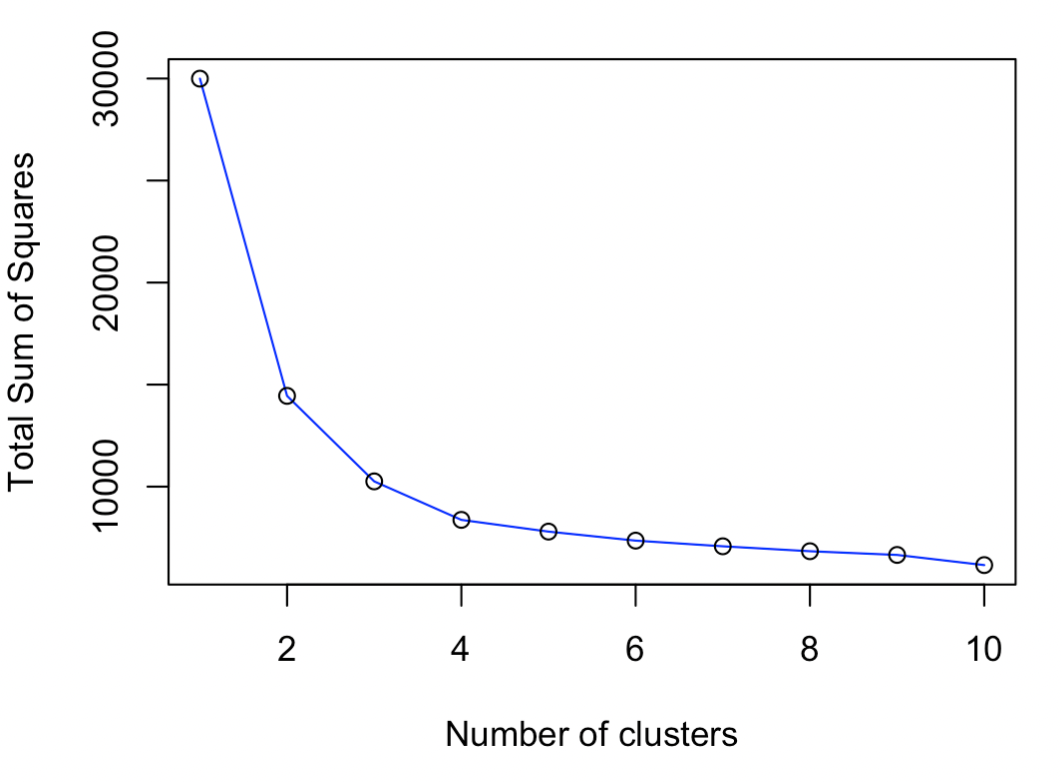
\includegraphics[width=0.5\linewidth]{elbowgraph}
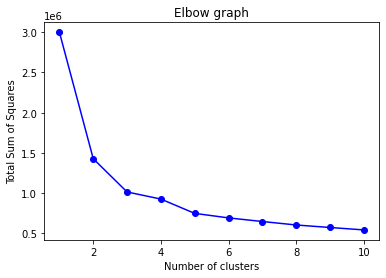
\includegraphics[width=0.5\linewidth]{elbowgraphPython}

In the graphs it can be seen that the elbow point, that is the point
where the graph presents an ``elbow'' due to a significant change in
slope, is associated with k = 2, so the optimal number of clusters for
our dataset will be 2, as we mentioned before.

\hypertarget{plot-the-first-2-dimensions-of-the-clusters}{%
\subsubsection{1.6. Plot the first 2 dimensions of the
clusters}\label{plot-the-first-2-dimensions-of-the-clusters}}

If we represent the first two dimensions of our dataset, ``price'' and
``speed'', for the two clusters created previously with the
``custom\_kmeans'' function, we obtain the following graphs, in both R
and Python:

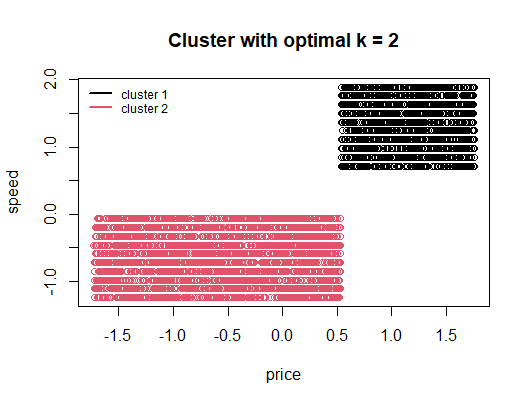
\includegraphics[width=0.5\linewidth]{first2dimensions}
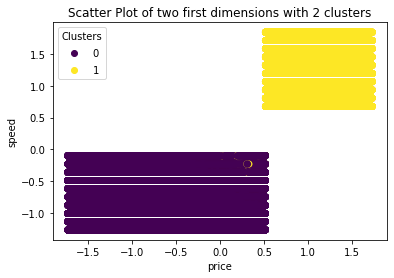
\includegraphics[width=0.5\linewidth]{first2dimensionsPython}

Despite the fact that two dimensions are too few to determine the
clusters of a dataset of six variables, we can observe that when we
graph these two variables together, two differentiated groups of data
are formed that correspond practically 100\% with the clusters that we
have created, which gives us an idea that our clusters are probably an
optimal solution for our dataset.

As we have said, two dimensions are not enough to appreciate the true
nature of the clusters, so in the following image we have decided to
plot the first three PCA of our dataset for our two clusters, in order
to observe them better:

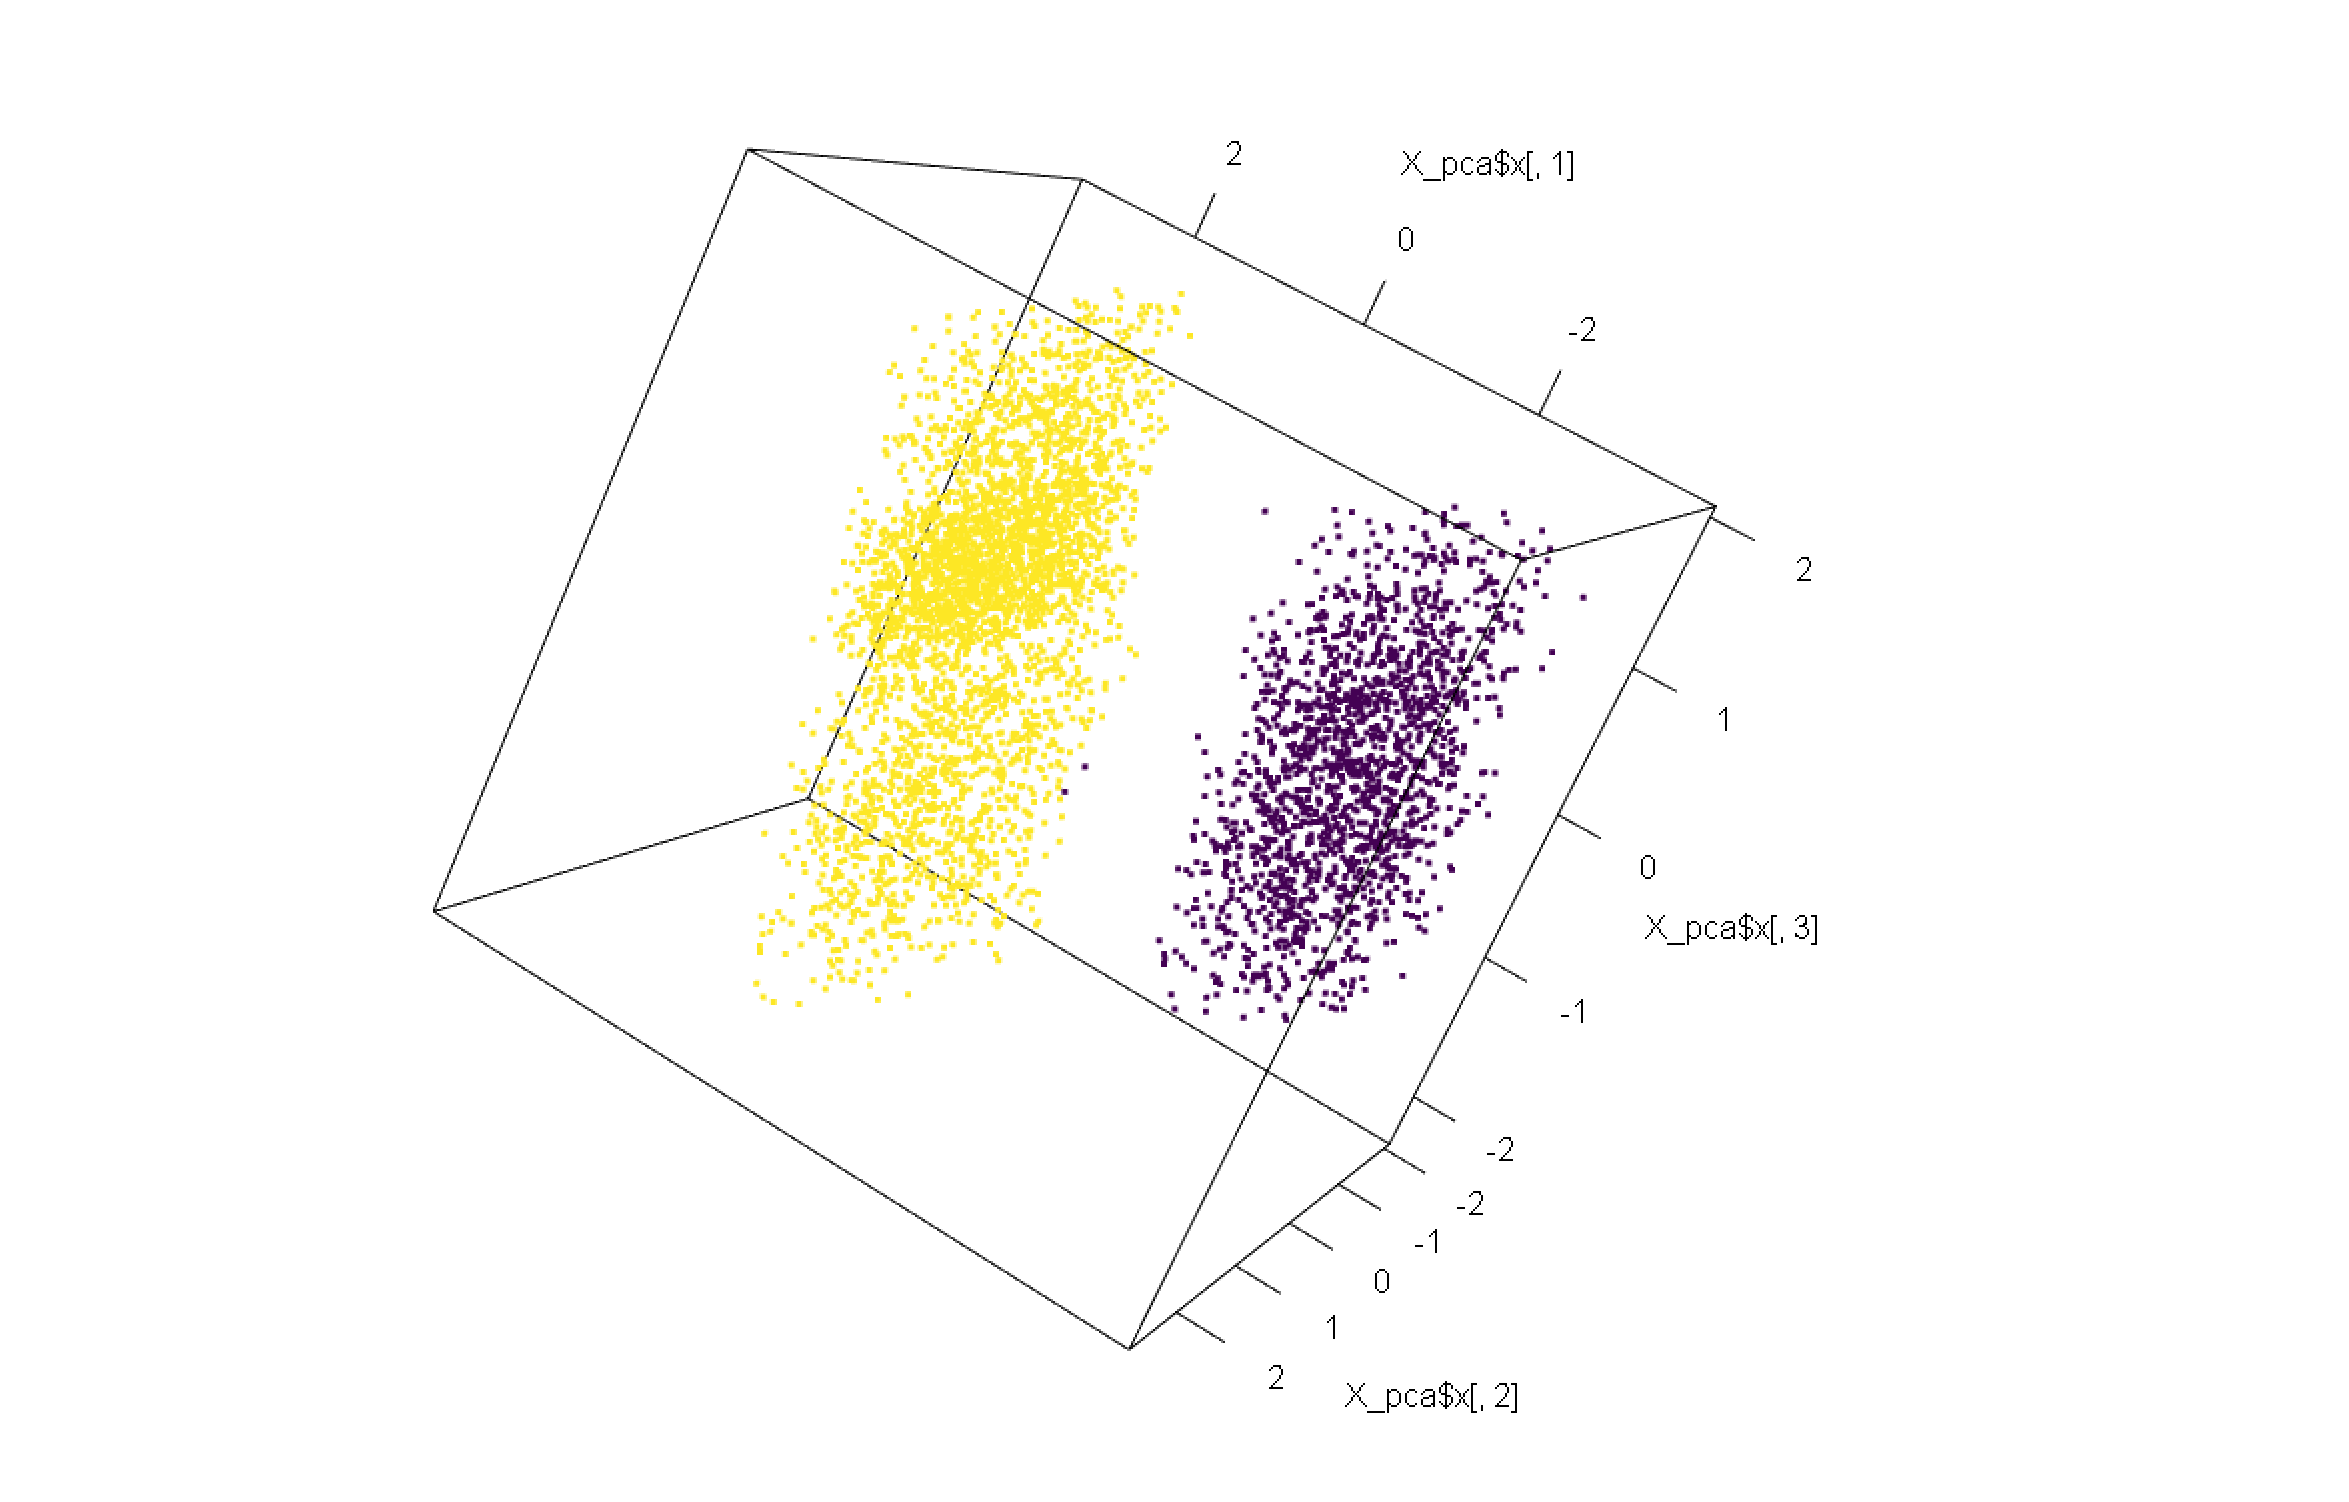
\includegraphics[width=1\linewidth]{3firstpca}

In this graph we can observe two different groups of data that again
correspond almost 100\% with our clusters, which again leads us to the
conclusion that we have created optimal clusters already suitable for
our dataset.

\hypertarget{find-the-cluster-with-the-highest-average-price-and-print-it}{%
\subsubsection{1.7. Find the cluster with the highest average price and
print
it}\label{find-the-cluster-with-the-highest-average-price-and-print-it}}

After calculating the average price of both clusters, we have obtained
that the cluster with the highest average price is cluster 1, as we had
already been able to observe when we plotted the variables ``price'' and
``speed'' for our two clusters.

\hypertarget{print-a-heat-map-using-the-values-of-the-clusters-centroids}{%
\subsubsection{1.8. Print a heat map using the values of the clusters
centroids}\label{print-a-heat-map-using-the-values-of-the-clusters-centroids}}

Next we have created a heat map using the values of the clusters
centroids, in both R and Python:

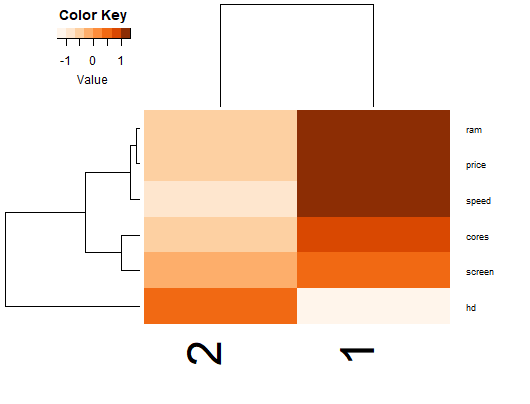
\includegraphics[width=0.5\linewidth]{heatmap}
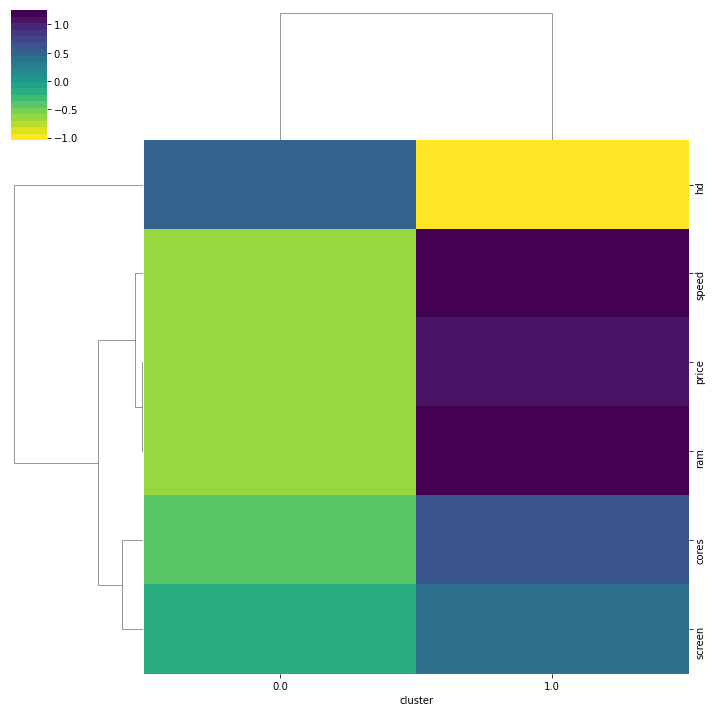
\includegraphics[width=0.5\linewidth]{heatmapPython}

In this graphs we can observe the dependency of belonging to each
cluster depending on each of the variables of the dataset. Cluster 1 is
characterized as having the highest average for ``ram'', ``price'',
``speed'', ``cores'' and ``screen'', while cluster 2 has the highest
average for ``hd''.

\hypertarget{parallel-implementation-multiprocessing}{%
\subsection{2. Parallel implementation,
multiprocessing}\label{parallel-implementation-multiprocessing}}

\hypertarget{write-a-parallel-version-of-you-program-using-multiprocessing}{%
\subsubsection{2.1. Write a parallel version of you program using
multiprocessing}\label{write-a-parallel-version-of-you-program-using-multiprocessing}}

\hypertarget{measure-the-time-and-optimize-the-program-to-get-the-fastest-version-you-can}{%
\subsubsection{2.2. Measure the time and optimize the program to get the
fastest version you
can}\label{measure-the-time-and-optimize-the-program-to-get-the-fastest-version-you-can}}

\hypertarget{plot-the-first-2-dimensions-of-the-clusters-1}{%
\subsubsection{2.3. Plot the first 2 dimensions of the
clusters}\label{plot-the-first-2-dimensions-of-the-clusters-1}}

\hypertarget{find-the-cluster-with-the-highest-average-price-and-print-it-1}{%
\subsubsection{2.4. Find the cluster with the highest average price and
print
it}\label{find-the-cluster-with-the-highest-average-price-and-print-it-1}}

\hypertarget{print-a-heat-map-using-the-values-of-the-clusters-centroids-1}{%
\subsubsection{2.5. Print a heat map using the values of the clusters
centroids}\label{print-a-heat-map-using-the-values-of-the-clusters-centroids-1}}

\hypertarget{parallel-implementation-threading}{%
\subsection{3. Parallel implementation,
threading}\label{parallel-implementation-threading}}

\hypertarget{write-a-parallel-version-of-you-program-using-threads}{%
\subsubsection{3.1. Write a parallel version of you program using
threads}\label{write-a-parallel-version-of-you-program-using-threads}}

\hypertarget{measure-the-time-and-optimize-the-program-to-get-the-fastest-version-you-can-1}{%
\subsubsection{3.2. Measure the time and optimize the program to get the
fastest version you
can}\label{measure-the-time-and-optimize-the-program-to-get-the-fastest-version-you-can-1}}

\hypertarget{plot-the-first-2-dimensions-of-the-clusters-2}{%
\subsubsection{3.3. Plot the first 2 dimensions of the
clusters}\label{plot-the-first-2-dimensions-of-the-clusters-2}}

\hypertarget{find-the-cluster-with-the-highest-average-price-and-print-it-2}{%
\subsubsection{3.4. Find the cluster with the highest average price and
print
it}\label{find-the-cluster-with-the-highest-average-price-and-print-it-2}}

\hypertarget{print-a-heat-map-using-the-values-of-the-clusters-centroids-2}{%
\subsubsection{3.5. Print a heat map using the values of the clusters
centroids}\label{print-a-heat-map-using-the-values-of-the-clusters-centroids-2}}

\end{document}
